\documentclass[12pt]{article}
\usepackage{graphicx}
\usepackage{fancyhdr}
\usepackage[hidelinks]{hyperref}
\usepackage{wrapfig}
\usepackage[sort]{cite}
\usepackage{url}
%\usepackage[left=20mm,top=20mm,bottom=20mm,right=20mm]{geometry}

\begin{document}
\author{Teun Kokke, s1242775}
\title
{
	\vspace*{\dimexpr-1.4in-\topmargin-\headsep-\headheight-\baselineskip}%
	\hspace*{\dimexpr-1.2in-\evensidemargin-\parindent}%
	\makebox[\paperwidth][r]{
\includegraphics[height=3cm]{logo.png}}
    Rendonan Minigame\\
    {\small Software Engineering Large Practical\\Word Count: xxxxx}
    \vspace{18em}
}

\begin{titlepage}
\maketitle
\end{titlepage}

\section*{QUESTIONS TO SUPERVISOR}
\begin{itemize}
\item Need to mention examples in background for "why gamemaker"? if no, where should examples be given if at all?
\item Known from previous experiments: a single instance cannot simulate more than roughly 700 clients without causing losing stability. Do I have to show this in detail with a graph as part of the experiments, or should I just mention that eg. 500 clients per instance is arbitrary for this reason and ignore the details?
\item Is it required to include formulae for mean, variance and standard-deviation?
\end{itemize}

\section*{TODO}
\begin{itemize}
\item give definition for server-reponse time
\item in section "fairness depending on location", add world map with tested locations and their average mean
\end{itemize}

\section*{Abstract}
Creating an extention for Gamemaker creations, to allow fast networking with maximal reliability.
\pagebreak

\tableofcontents
\pagebreak

\part{Preamble}
\pagebreak

\section{Introduction}

\section{Background}
%intro and synopsis (topic description and setting context of published literature, main results summarized.. about 5 pages)
%- summary of ALL contributions, code, research interpretations, tests, experiments (bulleted list)

\subsection{HTML5}

\paragraph{}HTML5 was released in 2014 (October 28th) by the World Wide Web Consortium (W3C) and is a raising web standard, improving its predecessor HTML4 with the aim to reduce the dependence of functionality from third-party plugins such as Flash and Java applets, which are deprecated and unsupported by many devices\footnote{http://i-programmer.info/news/86-browsers/8783-death-of-flash-and-java.html}.
\paragraph{}Scripting is replaced in HTML5 by markup where-ever possible, causing the world of browser-gaming to change rapidly. One of the the newly introduced features is the <canvas> tag, giving rise to isometric JavaScript applications.


\subsection{NodeJS}
NodeJS \footnote{http://www.toptal.com/nodejs/why-the-hell-would-i-use-node-js}
\paragraph{}

\subsection{GameMaker}
\subsection{Environmental Psychology}
\subsection{Networks in applications}
\subsection{The full picture}
\paragraph{}Gamemaker by YoyoGames is a software creation tool with the aim to simplify and speed up game and app development. It is cheap, simple to learn and flexible to use, making the software demanded by small teams, professionals and novice developers. Consequently, the human nature of staying within trusted environments causes developers to stick to Gamemaker.

\paragraph{}During the rise of HTML5 and the growing popularity of the Gamemaker, YoyoGames has provided the functionality to export any application to a JavaScript program that can be executed directly in the browser. This way i.a. updates can be made seamless, require no file-download nor installation, is platform-independent and easier to distribute.

\paragraph{}Some features are lost during the transition from a windows-executable to a web-application. One of them is a critical component to application popularity: networking functionality. Since the HTML5 update in September 2011, this feature was never added.
\paragraph{} The implementation in this Honours project will allow developers to again add networking features to their web-browser applications.

\pagebreak
\part{Literature Review}
\pagebreak

\section{Networks}
\subsection{OSI layers and Protocols}
%how to imagine the path data has to travel
\subsection{Inter-application communication}
%how do applications communicate
%IMPORTANT: State why there is no need for testing fairness between different bandwidths for web applications. (ie. games and web-apps only really need to send small variables, no big data is transported)

\section{Network benchmark criteria}
%which criteria to consider when testing a network
\subsection{Target audience}
%explain the types of target audience, who do the developers of an application using the extension intend to target. How does this affect the demands on the network
%focus on location of users

\subsection{Minimal requirements}
%minimal requirements for a network for a proper user experience
http://drewww.github.io/socket.io-benchmarking/
\\http://blog.mixu.net/2011/11/22/performance-benchmarking-socket-io-0-8-7-0-7-11-and-0-6-17-and-nodes-native-tcp/

\section{Socket.io "under the hood"}
%benchmarks for socket.io made by other developers

\pagebreak
\part{Implementation}
%discussion of work undertaken, sub-problems, solutions, difficulties
%\\- concentrated discussions for implementation principles and aspects
%\\- clarify WHAT WAS COMPLETED, and what wasnt.
\pagebreak
\section{Design}
\subsection{Project layout and prior considerations}
\subsection{Server and client}
\subsection{Creating applications}
\subsubsection{Benchmark application}
%Explain about ownmade application using the extension, how it tests the given benchmarks (eg. delay, data, equality)
\subsubsection{Real test application}
%Explain about ownmade test application representing a real game / program, made for observing user experience of the network for games developed with the extension.
\subsubsection{Templates for developers}
%How to make it easy for other developers to create applications with the extension. eg. Creating templates

%project layout. client, server, benchmark application, equality application, user experience

\section{The extension}

\section{Mapping from GML to the extension}

\section{Receiving and handling data at the server}


\pagebreak
\part{Experiments}
%description of experiments, presentation + interpretation of the data
\pagebreak

\section{Setup}
%explain every detail of how the experiments were setup, how everything worked.
Found people across the globe to assist in testing, family, friends and people found through social media, the Dutch gamemaker community and the Yoyogames forums.
\begin{itemize}
\item All network experiments are executed on a single server located in Edinburgh.
\item In each experiment all clients were connected and communicating to the server simultaneously.
\end{itemize}
%Note: add reminder that developers can setup peer-to-peer network by using the extension to serve as both server and client in their client application, but that these tests specifically consider the strength of each individual application acting as server.
\subsection{Server hardware and network specification}
\begin{itemize}
\item Node v0.12.3
\item Socket.io v1.3.7

\item Windows 7, SP 1
\item 64-bit platform
\item Intel(R) Core(TM) i7-2600K CPU @ 3.40GHz, 3401Mhz, 4 Cores (8 Logical Processors)
\item 12.6GB Available Physical Memory

\item 54.0Mb/s download
\item 3.0Mb/s upload
\end{itemize}

\section{Controlled Environment}
%testing in dummynet with specified setups
\subsection{Considerations}
\begin{itemize}
\item Server performance with regard to the number of concurrent connections.
\item The number of messages that can be handled by the server simultaneously.
\item The effect on server response-time of geographic distance between the client and server.
\item Fairness in server response-time between individual clients
\end{itemize}

\paragraph{Network Configuration}
\begin{itemize}
\item The network assumes no packet losses.
\item The network in-pipe is set to 10ms delay and a 5Mbit/s connection.
\item The network out-pipe is set to 10ms delay and a 5Mbit/s connection.
\end{itemize}



\subsection{Stress tests}

\subsubsection{Concurrent connections}
\paragraph{Environment}
\begin{itemize}
\item Variable number of concurrent connections cc, up to 15 instances with each simulating at most 500 clients.
\item Clients do not contact the server after establishing a connection.
\end{itemize}

\paragraph{Records}
\begin{itemize}
\item CPU usage on the server
\item CPU time on the server
\item Resident set size (RSS) on the server
\end{itemize}

\paragraph{Results}\mbox{}\\\\

\begin{center}

\begin{figure}
% \centering% default with `floatrow`
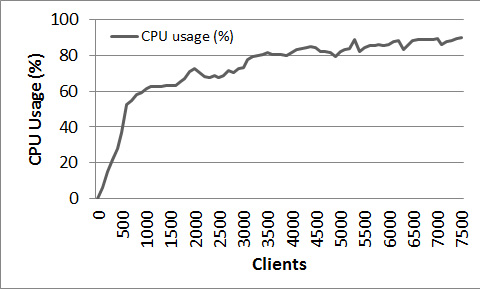
\includegraphics[scale=0.75]{test_CLIENT_CPUusage.jpg}
\caption{Displaying the CPU usage for the server process in percent.}
\vspace{1em}
When the CPU usage is above 70 percent, the user may experience lag. Such high CPU usage indicates insufficient processing power. Either the CPU needs to be upgraded, or the user experience reduced 
\footnote{\url{https://en.wikipedia.org/wiki/CPU_time}}
\end{figure}


\begin{figure}
% \centering% default with `floatrow`
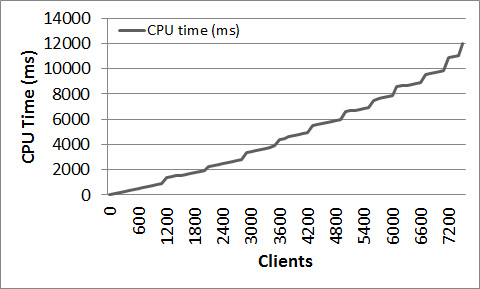
\includegraphics[scale=0.75]{test_CLIENT_CPUtime.jpg}
\caption{CPU time in milliseconds, displaying the amount of time required for the server to process the clients.}
\end{figure}


\begin{figure}
% \centering% default with `floatrow`
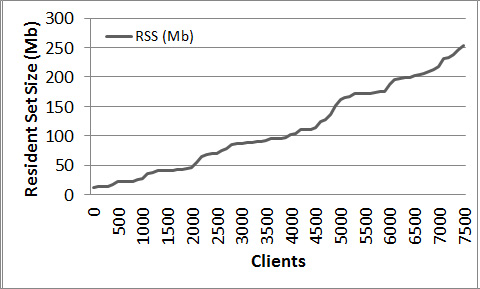
\includegraphics[scale=0.75]{test_CLIENT_RSS.jpg}
\caption{Resident set size in Megabit, showing the portion of RAM that is occupied by the server process.}
\end{figure}

\end{center}


\subsubsection{Message handling performance}
\paragraph{Environment}
\begin{itemize}
\item 5000 concurrent connections (10 instances each simulating 500 clients)
\item Each client sends 8-byte packages
\item Each client sends a variable number n of packages per second.
\item Each package roundtrip time is measured
\end{itemize}

\paragraph{Records}
\begin{itemize}
\item Mean roundtrip time between all clients
\item Deviation in roundtrip time between all clients
\end{itemize}

\paragraph{Results}

\section{Real Network Delay and Fairness}
%testing the extension in real networks

\subsection{Fairness depending on location}
For this experiment, multiple tests were executed with clients being located at specified locations. In each case, the clients were sending 8-byte messages to the server at a regular interval of 1 second for 2 minutes. The 120 roundtrip times for each client were then averaged in order to blur occasional peaks. At this point the roundtrip times of the clients in each common location were averaged, and then the deviance of the roundtrip times at each of these locations were calculated.

\paragraph{Test cases:}
\begin{enumerate}
\item Local network setting: Five clients physically located in the same local home network.

\item Same city: Five clients physically located in Edinburgh (LAN excluded).

\item Same country: Three clients physically located in Scotland: Edinburgh, Glasgow and Dundee.

\item Europe: Five clients physically located in the United Kingdom, Hungary, France, Germany and the Netherlands.

\item Inter-continental: Eight clients physically located in South Africa, California (USA), India, Thailand, Germany, Hungary, United Kingdom and the Netherlands.

\end{enumerate}

\paragraph{Results:}Average roundtrip times per location:
\begin{center}
  \begin{tabular}{ r | l }
Location		& Average RTT \\ \hline\hline
LAN				& 32ms	\\
Edinburgh		& 55ms	\\
Dundee			& 65ms	\\
Germany			& 67ms	\\
Glasgow			& 68ms	\\
France			& 69ms	\\
the Netherlands	& 70ms	\\
United Kingdom	& 71ms	\\
Hungary			& 76ms	\\
India			& 103ms	\\
South Africa	& 144ms	\\
California (USA)& 158ms	\\
Thailand		& 171ms	\\
  \end{tabular}
\end{center}

Average roundtrip times per test:
\begin{center}
  \begin{tabular}{ | r || c | c | c | c | c |}
    \hline
    Test case 		& 1 		& 2 		& 3 		& 4 		& 5 		\\ \hline\hline
    Mean RTT 		& 32.1ms 	& 54.8ms 	& 62.7ms 	& 70.6ms 	& 107.5ms	\\ \hline
    Variance RTT 	& 1.3ms 	& 8.2ms 	& 46.3ms 	& 11.3ms 	& 1900.9ms	\\ \hline
    Std RTT			& 0.4ms		& 2.9ms		& 6.8ms		& 3.36ms	& 43.6ms	\\ \hline
  \end{tabular}
\end{center}







\section{Developer Friendliness}
%userfriendliness of the extension, how hard is it for other developers to use it?
\subsection{User Feedback}
%feedback from users given through forum

The project focus is on developing a networking extension, to allow the use of networking services to Gamemaker when using the HTML5 export option.\\
One of the first thing one would consider is the selection of protocols that will be used in order to establish the connection between two (or more) nodes.\\
As the project aims to allow users to optimise the extension's networking settings in favour of either speed or reliability, there will be further research done within each of the transport layer protocols: TCP and UDP.\\
One of the most immediate problems that arise are that due to security constraints, UDP is not normally supported by web-browsers in order to communicate data to other hosts, and communication via TCP may be too slow in case a developer wishes to create an application that relies on a fast connection between hosts.

In order to evaluate the efficiency of the networking extension, use Dummynet to setup a controlled environment.

\begin{enumerate}
\item Display \# of clients connected
\item Display \# of requests server needs to process per second
\item Ping server every x time
\item Log ping values, compare with other data
\item Store logs, evaluate
\end{enumerate}

tests executed:
\begin{enumerate}
\item 1) 
\end{enumerate}

\section{Interpretation of the data}

\section{Issues}
\begin{enumerate}
\item Gamemaker does \textbf{not} support networking for HTML5 (js) export
\item The current extentions that exist for gamemaker are limited to a basic use of TCP
\item Webbrowsers do not generally support the use of UDP.
\\Suggested methods are developing a java or flash applet, which will handle the networking features.
\\A recent technology called \emph{WebRTC} allows js to use UDP data transfer directly on the web-client, but security features  within the network make holepunching complicated.
\end{enumerate} 

\pagebreak
\part{Epilogue}
\pagebreak
\section{Evaluation}
\section{Conclusion}
%conclusion, main achievements, unsolved problems, direction for further work



\begin{thebibliography}{1}

  \bibitem{notes} John W. Dower {\em Readings compiled for History
  21.479.}  1991.

  \bibitem{impj}  The Japan Reader {\em Imperial Japan 1800-1945} 1973:
  Random House, N.Y.

  \bibitem{norman} E. H. Norman {\em Japan's emergence as a modern
  state} 1940: International Secretariat, Institute of Pacific
  Relations.

  \bibitem{fo} Bob Tadashi Wakabayashi {\em Anti-Foreignism and Western
  Learning in Early-Modern Japan} 1986: Harvard University Press.

\end{thebibliography}

\end{document}
